\documentclass{standalone}
\usepackage{mathpazo}
\usepackage{siunitx}
\usepackage[american voltages, american currents, american inductors]{circuitikz}
\newcommand*{\equal}{=}

\begin{document}
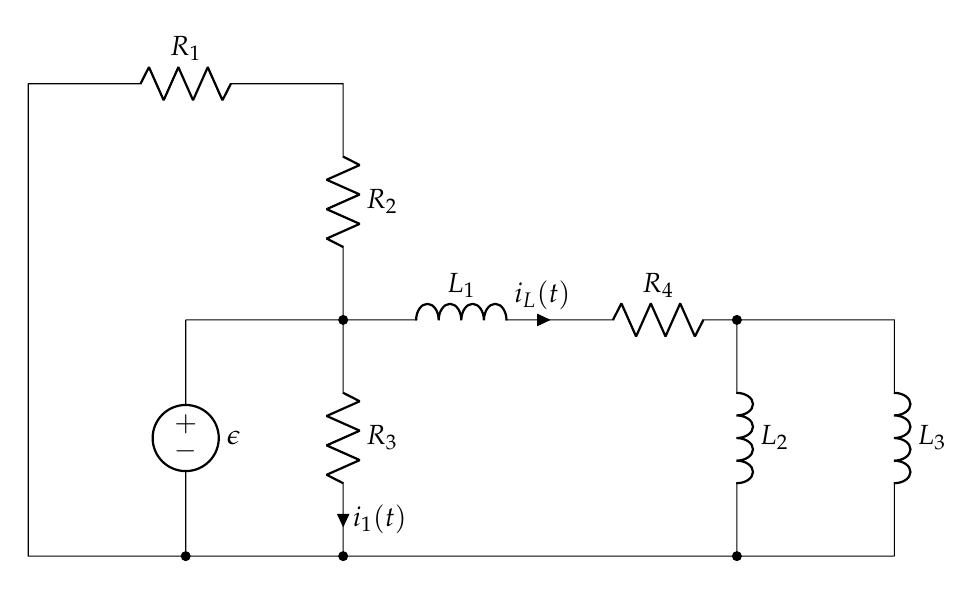
\begin{tikzpicture}
  \coordinate (A) at (0,6);
  \coordinate (B) at (0,0);
  \coordinate (C) at (4,6);
  \coordinate (D) at (4,3);
  \coordinate (E) at (4,0);
  \coordinate (F) at (9,3);
  \coordinate (G) at (9,0);
  \coordinate (H) at (11,3);
  \coordinate (I) at (11,0);
  \coordinate (J) at (2,3);
  \coordinate (K) at (2,0);
  \draw
  (J) to [short] (D)
  (J) to [V, l = $\epsilon$, -*] (K)
  (A) to [R, l = $R_1$] (C)
  to [R, l = $R_2$, -*] (D)
  to [R, l = $R_3$, -*, i = $i_1(t)$] (E)
  (D) to [L, l = $L_1$, i = $i_L(t)$] ++(3,0)
  to [R, l = $R_4$] (F)
  to [L, l = $L_2$, *-*] (G)
  (F) to  [short] (H)
  to [L, l = $L_3$] (I)
  (A) to [short] (B) to [short] (K) to [short] (I);
  \end{tikzpicture}
\end{document}